\documentclass[a4paper,10pt]{scrartcl}
\usepackage[utf8]{inputenc}
\usepackage{amsmath}
\usepackage{amssymb}
\usepackage{graphicx}
\usepackage{algpseudocode}
\usepackage{hyperref}

%opening
\title{Staggered grid}
\author{}

\begin{document}
\graphicspath{{./pictures/}}

\maketitle

% \begin{abstract}
% \end{abstract}

\tableofcontents
\newpage

\section{Balance equations}
\subsection{Mass balance equation}
\begin{equation}
 \begin{alignedat}{3}
 \frac{\partial \varrho}{\partial t} &+ \nabla \cdot (\varrho \textbf{v}) &&- q &= 0 \\[1em]
 \int_{V} \frac{\partial \varrho}{\partial t} \text{d} V &+ \int_{V} \nabla \cdot (\varrho \textbf{v}) \text{d} V &&- \int_{V} q \text{d} V &= 0 \\[1em]
 \int_{V} \frac{\partial \varrho}{\partial t} \text{d} V &+ \int_{\partial V} (\varrho \textbf{v}) \cdot \textbf{n} \text{d} \Gamma_{V} &&- \int_{V} q \text{d} V &= 0 \\[1em]
 \int_{V} \frac{\partial \varrho}{\partial t} \text{d} V &+ \int_{\partial V} \begin{pmatrix}\varrho u \\ \varrho v\end{pmatrix} \cdot \begin{pmatrix}n_1 \\ n_2\end{pmatrix} \text{d} \Gamma_{V}
   &&- \int_{V} q \text{d} V &= 0 \\[1em]
 \int_{V} \frac{\partial \varrho}{\partial t} \text{d} V &+ \int_{\partial V} [(\varrho u n_1) + (\varrho v n_2)] \text{d} \Gamma_{V}
   &&- \int_{V} q \text{d} V &= 0
\end{alignedat}
\end{equation}

\subsection{Momentum balance equation}
\begin{equation}
 \begin{alignedat}{6}
  \frac{\partial (\varrho \textbf{v})}{\partial t} &+ \nabla \cdot (\varrho \textbf{v} \textbf{v}^{\textup{T}}) &&- \nabla \cdot (\mu (\nabla \textbf{v} + \nabla \textbf{v}^{\textup{T}})) \\
    &+ \nabla p &&- \varrho \textbf{g} &&- \textbf{f} &&= 0 \\[2em]
  \int_{V} \frac{\partial (\varrho \textbf{v})}{\partial t} \text{d} V &+ \int_{V} \nabla \cdot (\varrho \textbf{v} \textbf{v}^{\textup{T}}) \text{d} V
    &&- \int_{V} \nabla \cdot (\mu (\nabla \textbf{v} + \nabla \textbf{v}^{\textup{T}})) \text{d} V \\
    &+ \int_{V} \nabla p \text{d} V &&- \int_{V} \varrho \textbf{g} \text{d} V &&- \int_{V} \textbf{f} \text{d} V &&= 0 \\[2em]
  \int_{V} \frac{\partial (\varrho \textbf{v})}{\partial t} \text{d} V &+ \int_{\partial V} (\varrho \textbf{v} \textbf{v}^{\textup{T}}) \cdot \textbf{n} \text{d} \Gamma_{V}
    &&- \int_{\partial V} (\mu (\nabla \textbf{v} + \nabla \textbf{v}^{\textup{T}})) \cdot \textbf{n} \text{d} \Gamma_{V} \\
    &+ \int_{\partial V} p \textbf{n} \text{d} \Gamma_{V} &&- \int_{V} \varrho \textbf{g} \text{d} V &&- \int_{V} \textbf{f} \text{d} V &&= 0
 \end{alignedat}
\end{equation}

\begin{equation}
 \textbf{v} \textbf{v}^{\textup{T}} = \begin{pmatrix}u u & u v \\ v u & v v \end{pmatrix}
\end{equation}
\begin{equation}
 \nabla \textbf{v} + \nabla \textbf{v}^{\textup{T}} =  \begin{pmatrix} 2 \frac{\partial u}{\partial x} & \frac{\partial u}{\partial y} + \frac{\partial v}{\partial x} \\
                                                        \frac{\partial v}{\partial x} + \frac{\partial u}{\partial y} & 2 \frac{\partial v}{\partial y}
                                                       \end{pmatrix}
\end{equation}

x-direction:
\begin{equation}
\begin{split}
  \int_{V} \frac{\partial (\varrho u)}{\partial t} \text{d} V + \int_{\partial V} (\varrho u u)n_1 + (\varrho u v)n_2 \text{d} \Gamma_{V} \\[1em]
    - \int_{\partial V} \left(\mu (2\frac{\partial u}{\partial x})n_1 + \mu (\frac{\partial u}{\partial y} + \frac{\partial v}{\partial x})n_2 \right) \text{d} \Gamma_{V} \\[1em]
    + \int_{\partial V} p n_1 \text{d} \Gamma_{V} - \int_{V} \varrho g_1 \text{d} V - \int_{V} f_1 \text{d} V = 0
\end{split}
\end{equation}

y-direction:
\begin{equation}
\begin{split}
  \int_{V} \frac{\partial (\varrho v)}{\partial t} \text{d} V + \int_{\partial V} (\varrho v u)n_1 + (\varrho v v)n_2 \text{d} \Gamma_{V} \\[1em]
    - \int_{\partial V} \left(\mu (\frac{\partial u}{\partial y} + \frac{\partial v}{\partial x})n_1 + \mu (2\frac{\partial v}{\partial y})n_2\right) \text{d} \Gamma_{V} \\[1em]
    + \int_{\partial V} p n_2 \text{d} \Gamma_{V} - \int_{V} \varrho g_2 \text{d} V - \int_{V} f_2 \text{d} V = 0
\end{split}
\end{equation}

\section{Scheme}
\subsection{Notation}
\begin{itemize}
 \item \textit{normal} and \textit{tangential/parallel}
 \begin{itemize}
  \item data: relating to the direction of the respective velocity (not the face direction), see figure \ref{fig:data_vertical_faces} and \ref{fig:data_horizontal_faces}
  \item assembly: relating to the respective face direction (normal flux = normal to face, parallel to velocity on respective face)
 \end{itemize}
 \item numbering of subfaces: view from cell center $\rightarrow$ left subface \textit{0}, right subface \textit{1}
 \item data pairs: dof belonging to the current element \textit{first}, dof belonging to the neighboring element \textit{second}
 \item gradients: dof[...second] - dof[...first] / time step
\end{itemize}

\begin{figure}
 \centering
 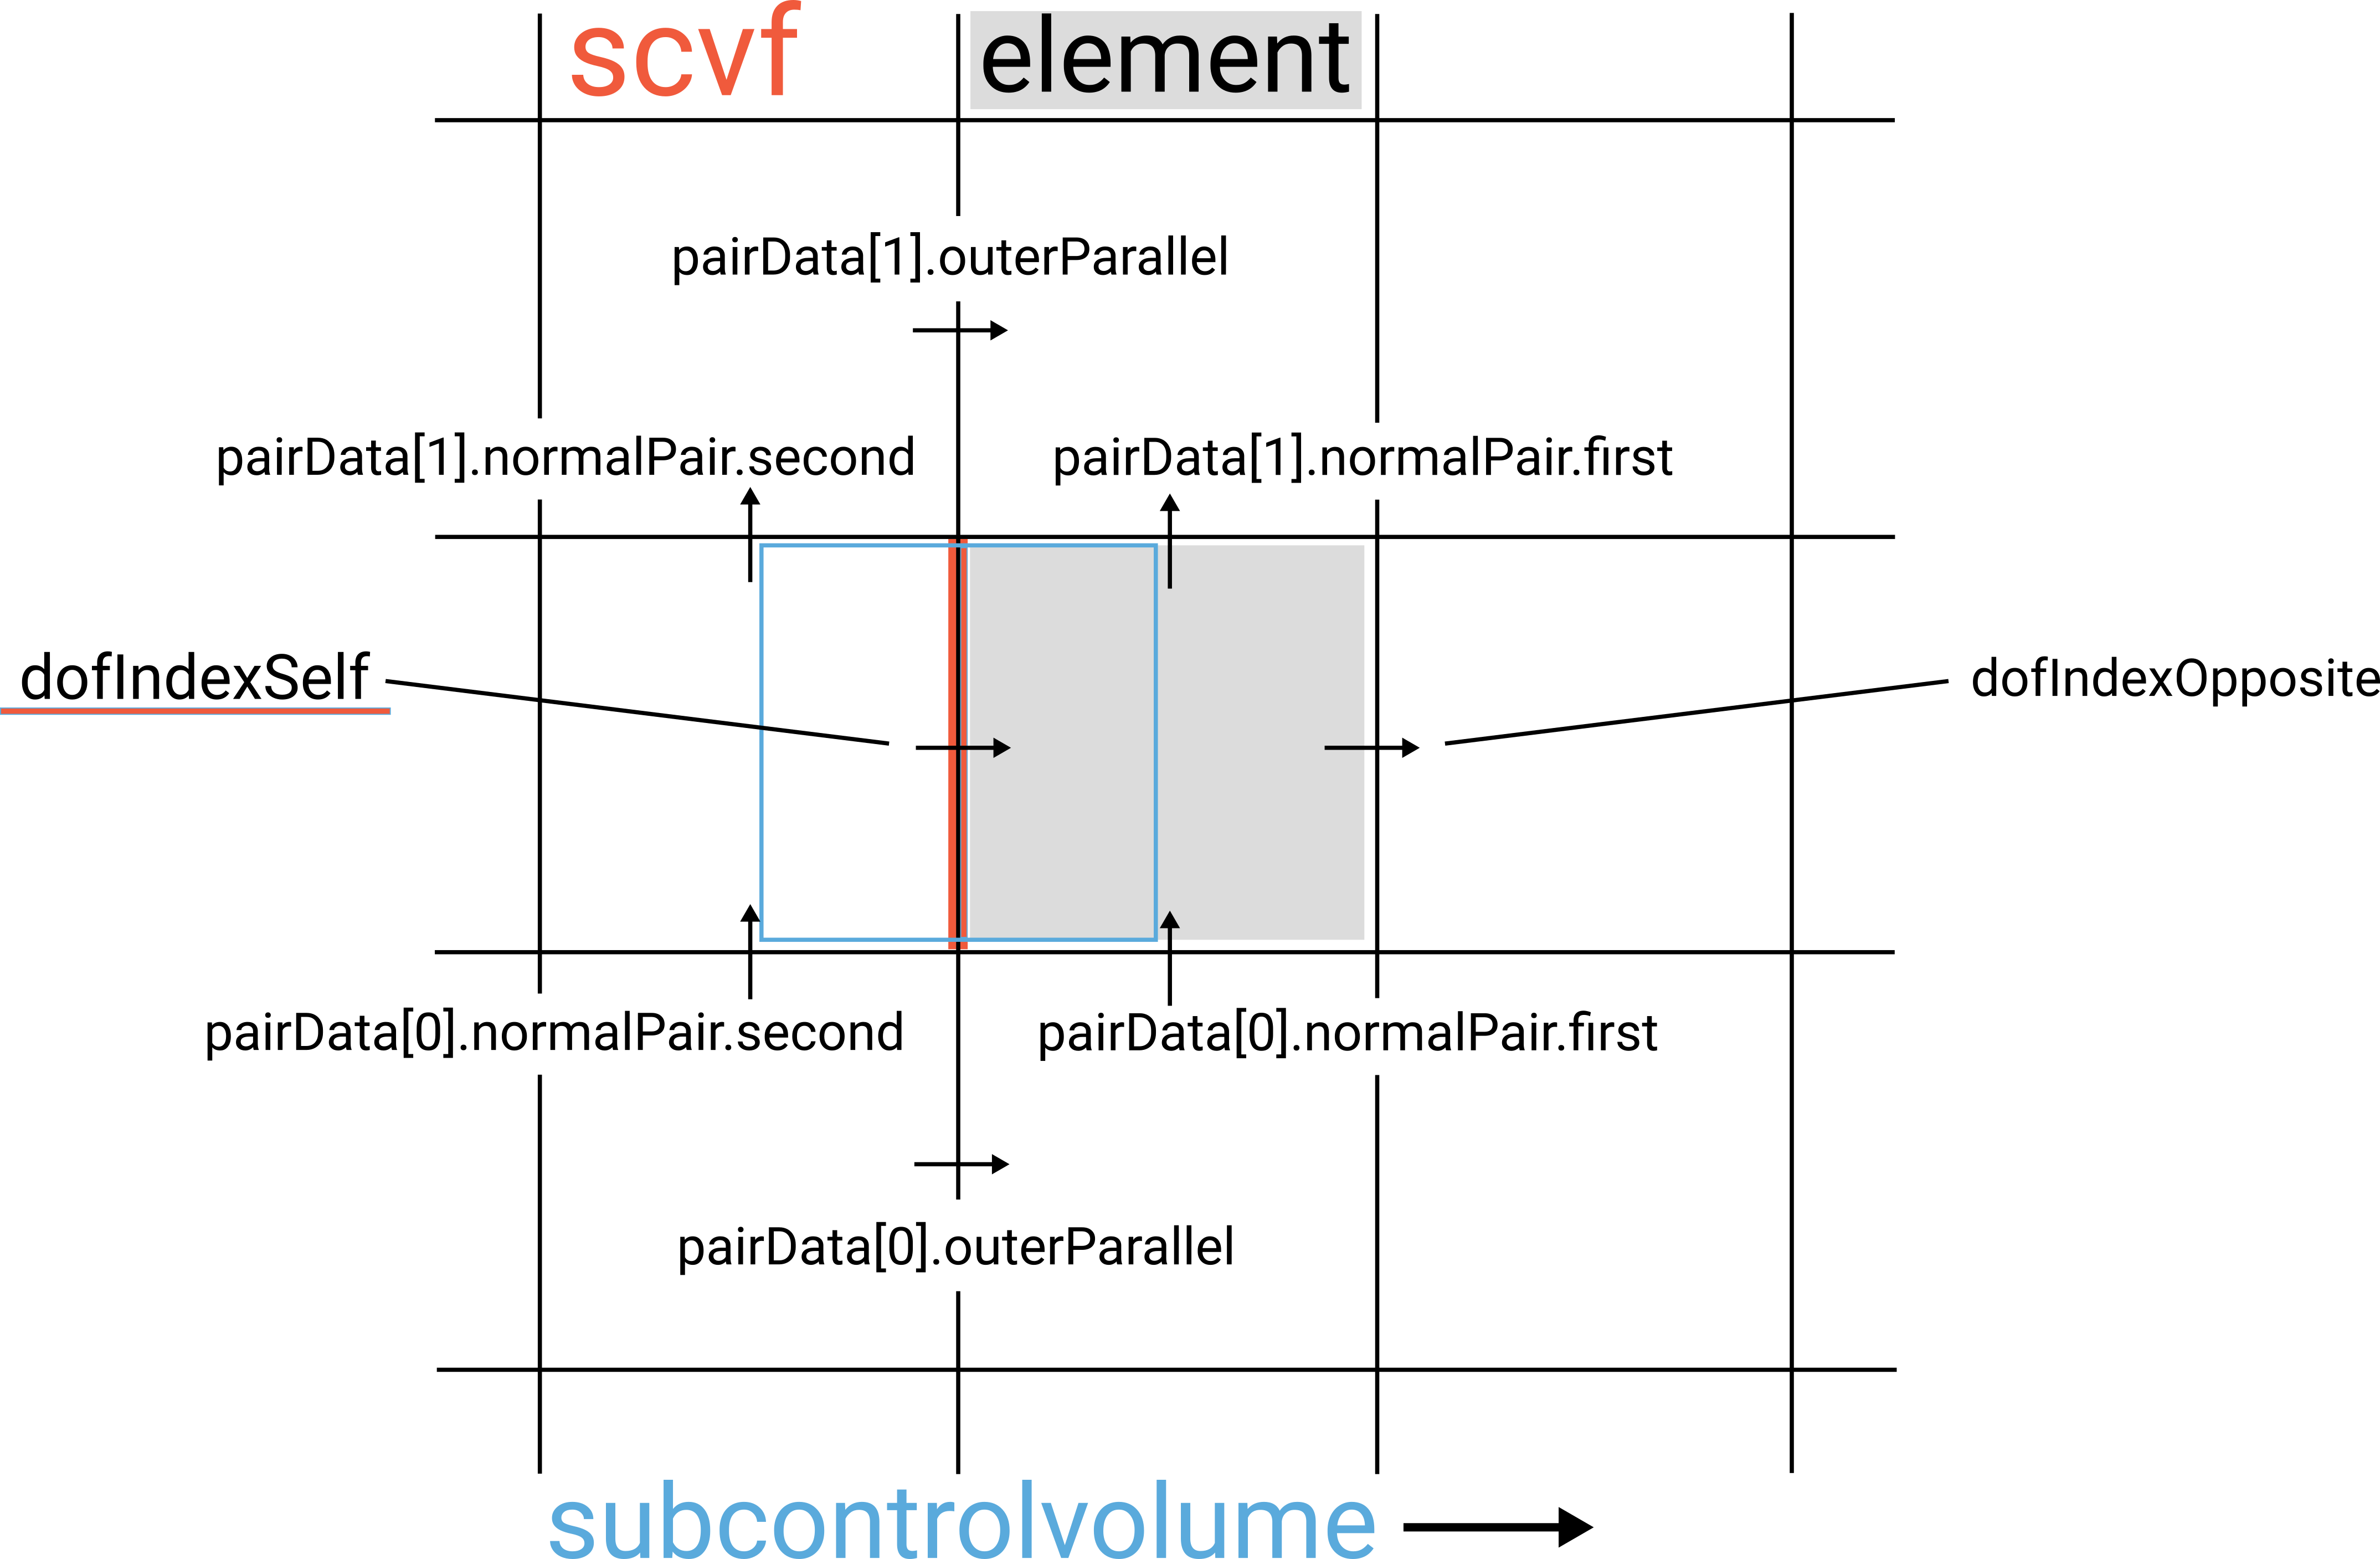
\includegraphics[width=0.8\textwidth]{scheme_scv_horizontal.png}
 \caption{Necessary data for computation of flux terms for vertical faces}
 \label{fig:data_vertical_faces}
\end{figure}

\begin{figure}
 \centering
 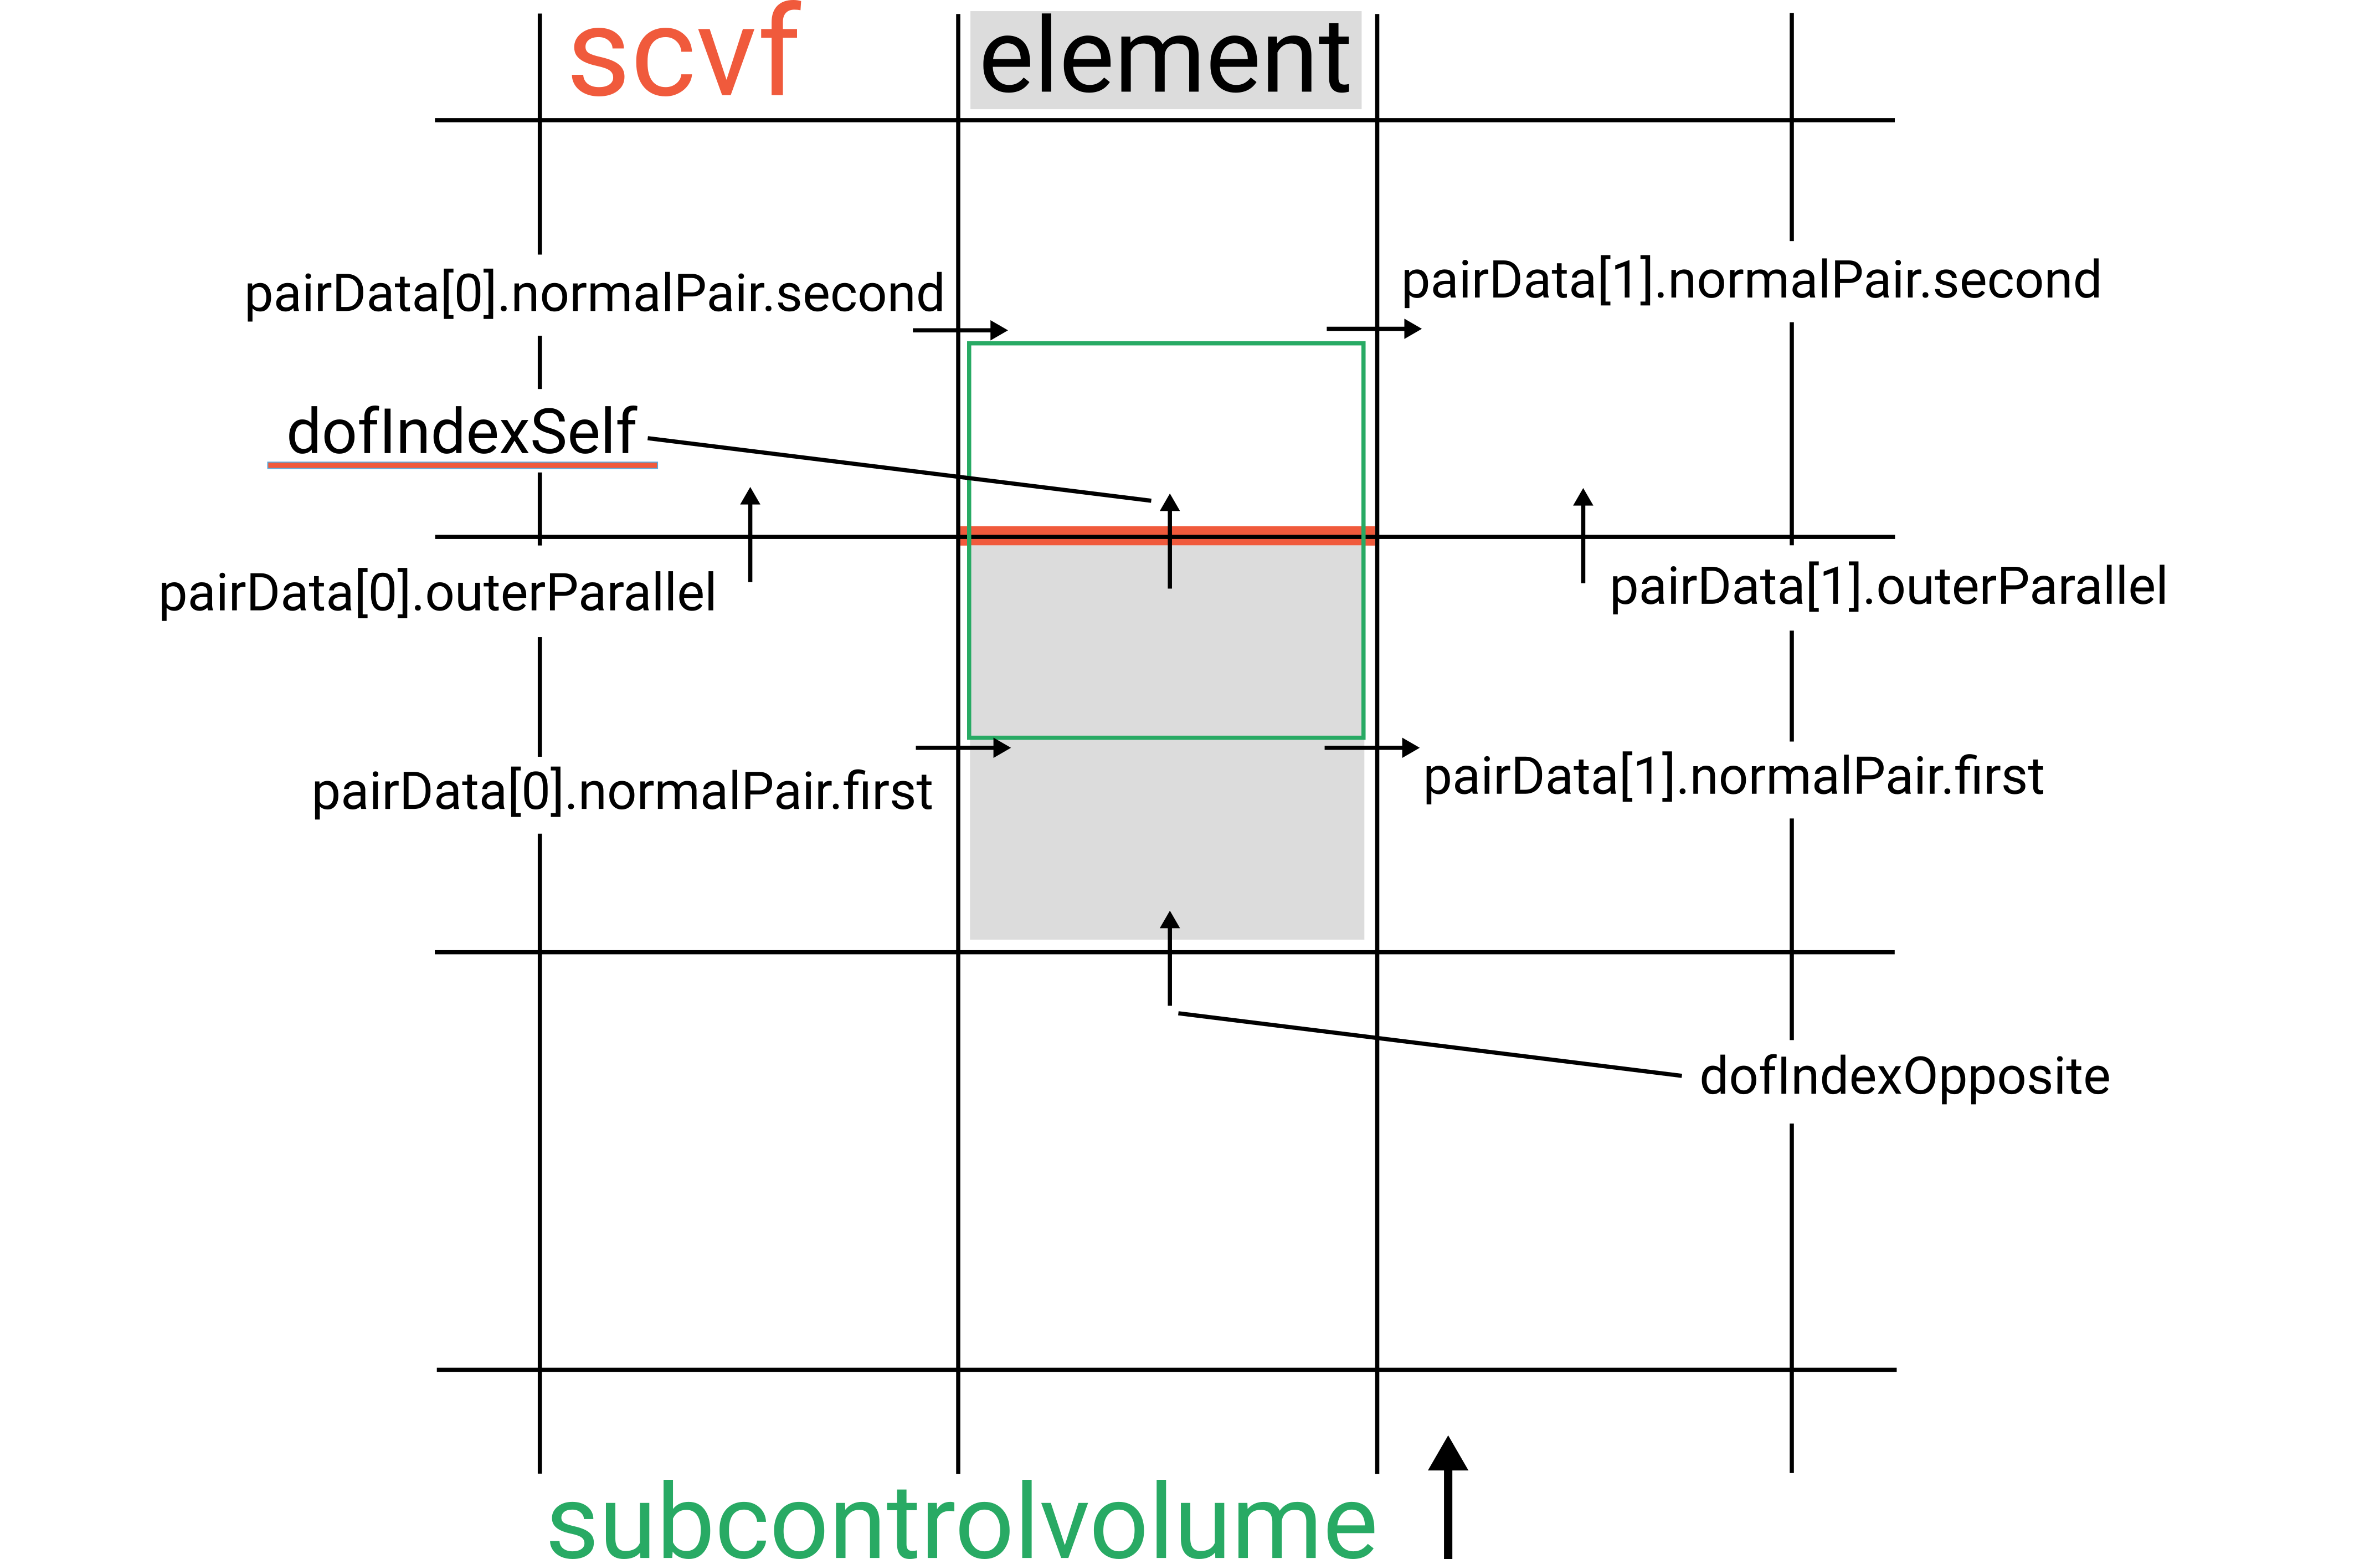
\includegraphics[width=0.8\textwidth]{scheme_scv_vertical.png}
 \caption{Necessary data for computation of flux terms for horizontal faces}
 \label{fig:data_horizontal_faces}
 \end{figure}
 
 \subsection{Implementation notes}
 \subsubsection{Residual}
 Local residual (element):
 \begin{center} residual\_ [ ][ ][ ] \end{center}
 \begin{itemize}
  \item 1st index: 0 $\rightarrow$ cell, 1 $\rightarrow$ face
  \item 2nd index: numCell/numFace (cell 0; face 0,1,2,3)
  \item 3rd index: numEq (cell 0,1,...; face 0)
 \end{itemize}
 $\Rightarrow$ Example for 2 dofs/cell, 1dof/face: \\
 pressure, temperature: residual\_[0][0][0], residual\_[0][0][1] \\
 velocities: residual\_[1][0][0], residual\_[1][1][0], residual\_[1][2][0], residual\_[1][3][0]. \\



\subsection{Algorithm}
% \begin{algorithmic}
%  \For{all elements}
%  \For{all faces} \\
%  get global index of the face itself (dofIndexSelf) \\
%  get global index of the opposite face (dofIndexOpposite) \\
%  get direction of face \\
%  \vspace{1em}
%   get index of upstream velocity (dofIndexUp) \\
%  v\_avg = (curVelocity(dofIndexSelf) + curVelocity(dofIndexOpposite)) / 2; \\
%  grad\_v = (velocity(dofIndexSelf) - velocity(dofIndexOpposite)) / \\ \hspace{2cm} selfToOppositeDistance; \\
%  \vspace{1em}
%  
%  ** compute volume terms ** \\
%  residual[dofIndexSelf] += (curVelocity(dofIndexSelf) * curDensity \\ \hspace{4cm}- prevVelocity(dofIndexSelf) * prevDensity) \\ \hspace{4cm} / deltaT * volume; \Comment storage \\
%  residual[dofIndexSelf] += curDensity * gravity(direction); \Comment gravity \\ \vspace{1em}
%  
%  ** compute normal terms **\\
%  residual[dofIndexSelf] += curDensity * v\_avg * velocity(dofIndexUp) \\ \hspace{4cm} * face.area * 0.5; \Comment advective term \\
%  residual[dofIndexSelf] -= 2 * mu * grad\_v * face.area * 0.5; \Comment viscous term \\ 
%  residual[dofIndexSelf] += pressure(element) * face.area * 0.5; \Comment pressure term \vspace{1em}
%  
%  ** compute tangential terms **
%  \For {all subfaces} \\
%  get innerElement, outerElement, innerVolVars, outerVolVars, innverVolume, outerVolume \\
%  get the upstream velocity, mu\_avg, upDensity \\ 
%  get gradSelf, gradNormal \\ \vspace{1em}
%  
%  residual[pairData[subface].normalPair.first] += upDensity * v\_avg * upVelocity \\ \hspace{6cm} * face.area * 0.5; \Comment advective term \\
%  residual[pairData[subface].normalPair.first] -= mu\_avg * (gradSelf + gradNormal) \\ \hspace{6cm} * face.area * 0.5; \Comment viscous term \\ 
%  \EndFor
%  \EndFor
%  \EndFor
%  
% \end{algorithmic}

\end{document}
